\documentclass[tikz,border=8pt]{standalone}
% Shared look for every TikZ diagram. Load with \input{../../tools/tikz-style.tex}
\usepackage[T1]{fontenc}
\usepackage{lmodern}
\renewcommand{\sfdefault}{lmr}  % diagrams use the same serif as the text
\usetikzlibrary{arrows.meta, positioning, shapes.geometric, calc, fit, backgrounds}
\definecolor{cblue}{HTML}{4C78A8}
\definecolor{corange}{HTML}{F58518}
\definecolor{cgreen}{HTML}{54A24B}
\definecolor{cred}{HTML}{E45756}
\definecolor{cpurple}{HTML}{B279A2}
\definecolor{cgrey}{HTML}{6B6B6B}
\tikzset{
  every picture/.style={font=\sffamily, line width=1.2pt},
  box/.style={draw=#1, fill=#1!12, rounded corners=4pt, align=center, inner sep=7pt, minimum height=1.1cm},
  box/.default=cgrey,
  arrow/.style={-{Stealth[length=3mm]}, draw=cgrey, line width=1.4pt},
  title/.style={font=\sffamily\bfseries\Large},
  note/.style={font=\sffamily\small, text=cgrey, align=center},
}
\AtBeginDocument{\hyphenpenalty=10000 \exhyphenpenalty=10000}

\begin{document}
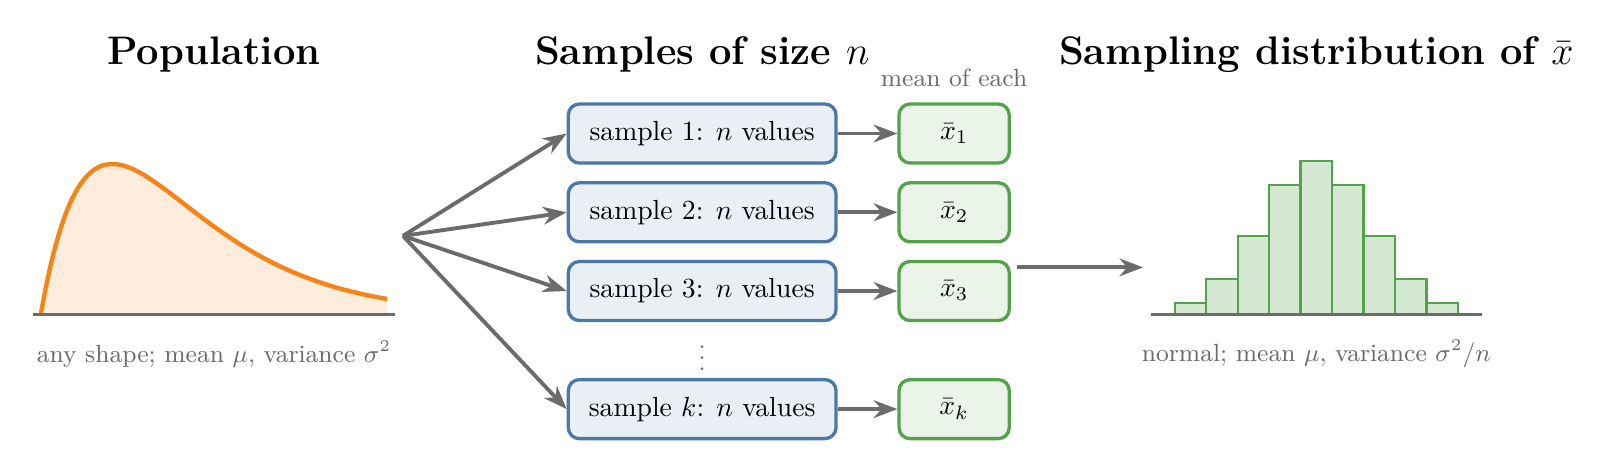
\begin{tikzpicture}
  % population: a right-skewed curve
  \node[title] at (0,3.3) {Population};
  \fill[corange!15] (-2.2,0) -- plot[domain=0:4.4, samples=80, smooth] ({\x-2.2},{2.6*\x*exp(-\x*1.1)*2.2}) -- (2.2,0) -- cycle;
  \draw[corange, line width=1.6pt] plot[domain=0:4.4, samples=80, smooth] ({\x-2.2},{2.6*\x*exp(-\x*1.1)*2.2});
  \draw[cgrey] (-2.3,0) -- (2.3,0);
  \node[note] at (0,-0.5) {any shape; mean $\mu$, variance $\sigma^2$};
  % samples
  \node[title] at (6.2,3.3) {Samples of size $n$};
  \foreach \i/\y in {1/2.3, 2/1.3, 3/0.3} {
    \node[box=cblue, minimum width=3.4cm, minimum height=0.75cm, inner sep=3pt] (s\i) at (6.2,\y) {sample \i: $n$ values};
    \node[box=cgreen, minimum width=1.4cm, minimum height=0.75cm, inner sep=3pt] (m\i) at (9.4,\y) {$\bar{x}_\i$};
    \draw[arrow] (s\i) -- (m\i);
    \draw[arrow] (2.4,1.0) -- (s\i.west);
  }
  \node[note] at (6.2,-0.45) {$\vdots$};
  \node[box=cblue, minimum width=3.4cm, minimum height=0.75cm, inner sep=3pt] (sk) at (6.2,-1.2) {sample $k$: $n$ values};
  \node[box=cgreen, minimum width=1.4cm, minimum height=0.75cm, inner sep=3pt] (mk) at (9.4,-1.2) {$\bar{x}_k$};
  \draw[arrow] (sk) -- (mk);
  \draw[arrow] (2.4,1.0) -- (sk.west);
  \node[note] at (9.4,3.0) {mean of each};
  % sampling distribution: bell-shaped histogram
  \node[title] at (14.0,3.3) {Sampling distribution of $\bar{x}$};
  \foreach \x/\h in {-1.6/0.15, -1.2/0.45, -0.8/1.0, -0.4/1.65, 0/1.95, 0.4/1.65, 0.8/1.0, 1.2/0.45, 1.6/0.15} {
    \fill[cgreen!25, draw=cgreen, line width=0.8pt] (14.0+\x-0.2,0) rectangle (14.0+\x+0.2,\h);
  }
  \draw[cgrey] (11.9,0) -- (16.1,0);
  \draw[arrow] (10.2,0.6) -- (11.8,0.6);
  \node[note] at (14.0,-0.5) {normal; mean $\mu$, variance $\sigma^2/n$};
\end{tikzpicture}
\end{document}
